\section{Thực hiện mạch đọc điện áp cho ngõ ra ADC}

\subsection{Tổng quan về ADC}

Theo chuẩn ngõ ra điện áp đọc từ Sensor là từ $0 \rightarrow 5\,\textsf{V}$, với ngõ vào là từ $20^{o}C \rightarrow 80^{o}C$ với bước nhảy là $0.1^{o}C$. Thực hiện tính giá trị của một bước nhảy nhỏ nhất là:

\[ \dfrac{5 - 0}{\dfrac{80 - 20}{0.1} + 1} \approx 8.3195 \,\textsf{mV} \]

Vậy có nghĩa là $\Delta_{min} \approx 8.3195 \,\textsf{mV} $, từ đó ta có:

\[ 2^{Q} = \dfrac{V_{ref^{+}} - V_{ref^{-}}}{\Delta_{min}} \]

Giả sử, chọn $V_{ref^{+}} = 5\,\textsf{V}$ và $V_{ref^{-}} = 0\,\textsf{V}$. Ta có $Q \approx 9.23\,\textsf{bit}$

Tuy nhiên, trong thị trường không có ADC $9.23\,\textsf{bit}$ cho nên nhóm em sẽ chọn con có trên thị trường là \href{https://www.ti.com/lit/ds/symlink/ads1115.pdf}{ADS1115IDGSR}.

\subsection{Electrical Characteristics của ADS1115}

\begin{itemize}[label=-]
	\item Ultra-small packages:
		\begin{itemize}[label=+]
				\item X2QFN: $2\,\textsf{mm} \times 1.5\,\textsf{mm} \times 0.4\,\textsf{mm}$
				\item SOT: $2.9\,\textsf{mm} \times 2.8\,\textsf{mm} \times 0.6\,\textsf{mm}$
		\end{itemize}
	
	\item Wide supply range: $2.0\,\textsf{V}$ to $5.5\,\textsf{V}$
	
	\item Low current consumption: $150\,\mu\textsf{A}$ (continuous-conversion mode)
	
	\item Programmable data rate: 8SPS to 860SPS
	
	\item Single-cycle settling
	
	\item Internal low-drift voltage reference
	
	\item Internal oscillator
	
	\item I2C interface: four pin-selectable addresses
	
	\item Operating temperature range: $-40^{o}C$ to $ + 125^{o}C$
	
	\item Family of devices:
		\begin{itemize}[label=+]
			\item ADS1115: four single-ended or two differential inputs with comparator and PGA
		\end{itemize}
\end{itemize}

Từ những thông tin, ADC ADS1115 có tầm hoạt động ở dải nhiệt độ phù hợp trong khoảng $20^{o}C \rightarrow 80^{o}C$, nhóm emm sử dụng nguồn cấp là $V_{DD} = 5.5\,\textsf{V}$ và cho phép nguồn sai số trong khoảng từ $[5.3, 5.5]\,\textsf{V}$ phù hợp với thông số dưới đây:

\begin{figure}[H]
	\centering
	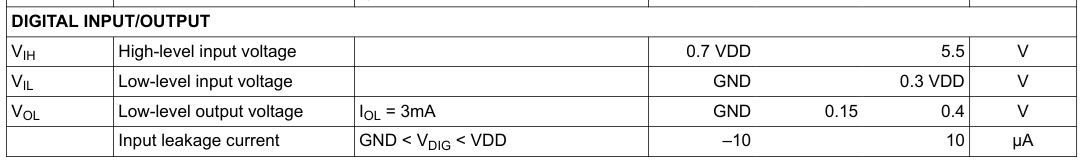
\includegraphics[width=.9\linewidth]{./my-chapters/my-images/ADC/datasheet_2.png}
	\caption{Digital Input/Output của ADS1115.}
\end{figure}

Như vậy, với $GND \approx 0\,\textsf{V} < V_{IN} < V_{DD} = 5.5\,\textsf{V}$ thì có thể phù hợp cho tầm đo từ $0 \rightarrow 5 \,\textsf{V}$ từ mạch đọc giá trị của sensor.

Tiếp theo, ta cần quan tâm đến giá trị như sau:
\begin{figure}[H]
	\centering
	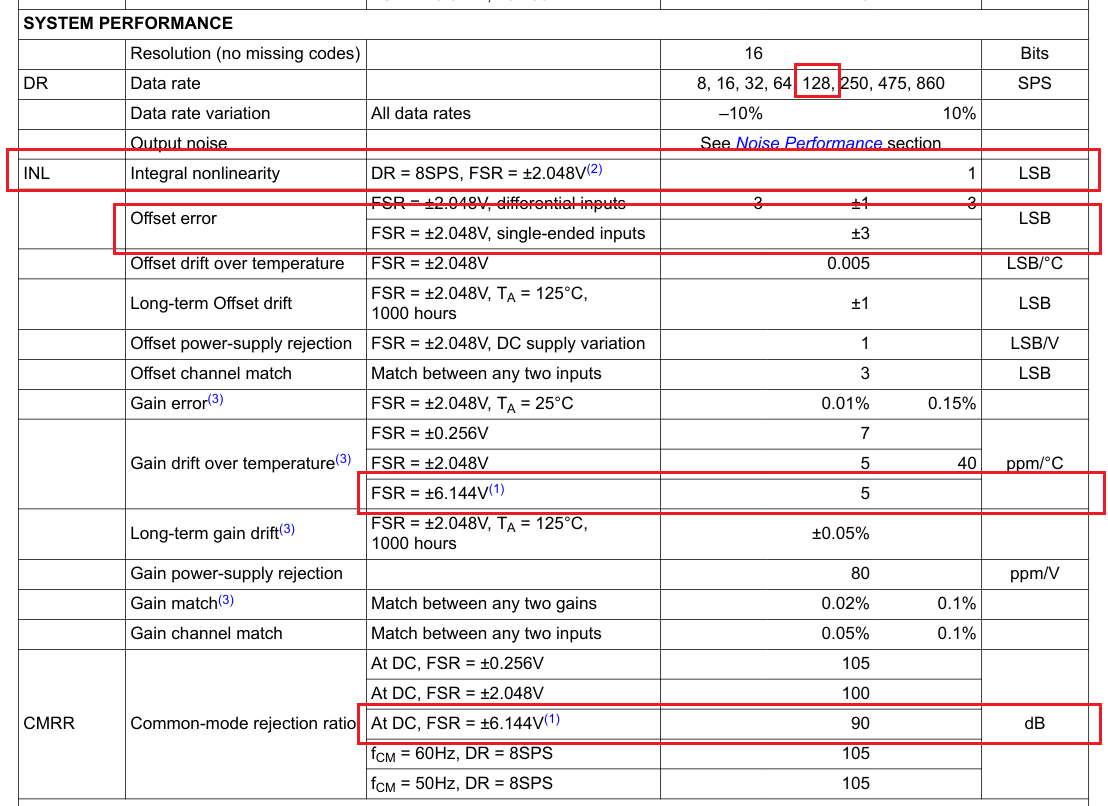
\includegraphics[width=.9\linewidth]{./my-chapters/my-images/ADC/datasheet_1.png}
	\caption{Electrical Characteristics của ADS1115.}
\end{figure}

\begin{itemize}[label=-]
	\item Data rate (DR) là giá trị dữ liệu Digital được đổi theo đơn vị thời gian.	Với $\textsf{DR} = 128$ Sample per second là giá trị default của ADS1115, với thời gian cách nhau đọc dữ liệu khoảng tầm $8\,\textsf{ms}$.
	\item Integral Nonlinearity (INL) là thước đo độ lệch của đặc tuyến chuyển đổi thực tế so với đặc tuyến lý tưởng trong các bộ chuyển đổi ADC/DAC, sau khi đã loại bỏ sai số offset và gain. Với $\textsf{INL} = 1\,\textsf{LSB}$.
	\item Offset error là sai số khi sử dụng chế độ Single-Ended với giá trị là $\pm 3\,\textsf{LSB}$.
	\item Gain drift over temperature là sai số của phép đo khi có ảnh hưởng của nhiệt độ với tại $\textsf{FSR} = \pm 6.144\,\textsf{V}$ thì Gain drift $= 5 ppm/^{o}C$ tức là mỗi $^{o}C$ sẽ gây sai số là $5$ phần ngàn.
	\item Common-mode Rejection Ratio (CMRR) là thước đo khả năng của một bộ khuếch đại vi sai trong việc loại bỏ tín hiệu chung xuất hiện đồng thời và cùng pha trên cả hai đầu vào. Với $\textsf{CMRR} = 90\,dB$.
\end{itemize}

\subsection{Typical Characteristics của ADS1115}

\begin{itemize}[label=-]
	\item Single-Ended Offset Error vs Temperature:
	
	\begin{minipage}{.5\linewidth}
		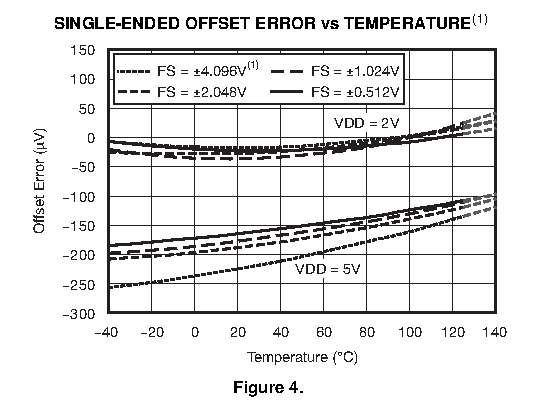
\includegraphics[width=\linewidth]{./my-chapters/my-images/ADC/datasheet_3.pdf}
	\end{minipage}
	\begin{minipage}{.5\linewidth}
		\begin{itemize}[label=+]
			\item Tại $T = 20^{o}C$: Offset Error $= -225\,\mu\textsf{V}$
			\item Tại $T = 80^{o}C$: Offset Error $= -120\,\mu\textsf{V}$
		\end{itemize}
	\end{minipage}
	
	\item Gain Error vs Temperature:
	
	\begin{minipage}{.5\linewidth}
		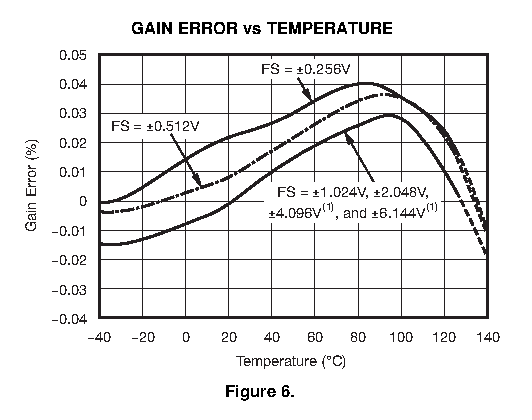
\includegraphics[width=\linewidth]{./my-chapters/my-images/ADC/datasheet_4.pdf}
	\end{minipage}
	\begin{minipage}{.5\linewidth}
		\begin{itemize}[label=+]
			\item Tại $T = 20^{o}C$: Gain Error $= 0.00\,\%$
			\item Tại $T = 80^{o}C$: Gain Error $= 0.03\,\%$
		\end{itemize}
	\end{minipage}
	
	\item Gain Error vs Supply:
	
	\begin{minipage}{.5\linewidth}
		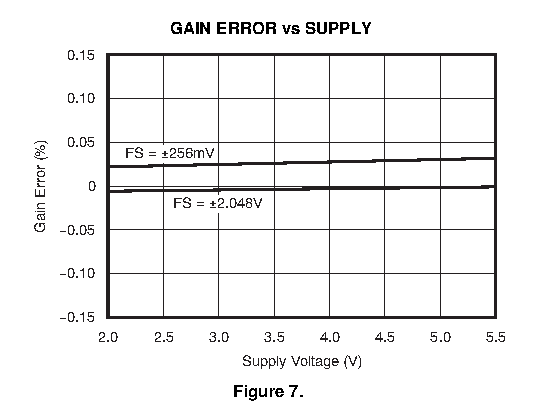
\includegraphics[width=\linewidth]{./my-chapters/my-images/ADC/datasheet_4_1.pdf}
	\end{minipage}
	\begin{minipage}{.5\linewidth}
		\begin{itemize}[label=+]
			\item Tại $V_{DD} = 5.5\,\textsf{V}$: Gain Error $= 0.00\,\%$
		\end{itemize}
	\end{minipage}
	
	\item INL vs Supply Voltage:
	
	\begin{minipage}{.5\linewidth}
		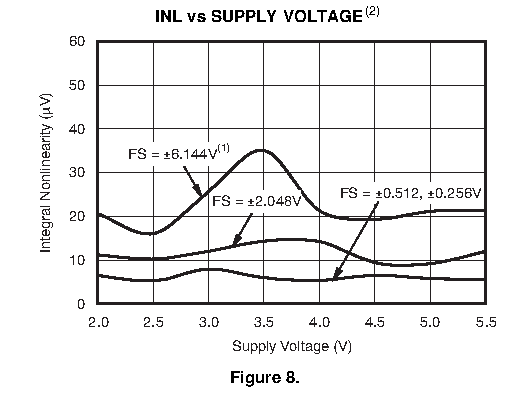
\includegraphics[width=\linewidth]{./my-chapters/my-images/ADC/datasheet_5.pdf}
	\end{minipage}
	\begin{minipage}{.5\linewidth}
		\begin{itemize}[label=+]
			\item Tại $V_{DD} = 5.5\,\textsf{V}$: INL vs Voltage $= 20\,\mu\textsf{V}$
		\end{itemize}
	\end{minipage}
	
	\item INL vs Temperature:
	
	\begin{minipage}{.5\linewidth}
		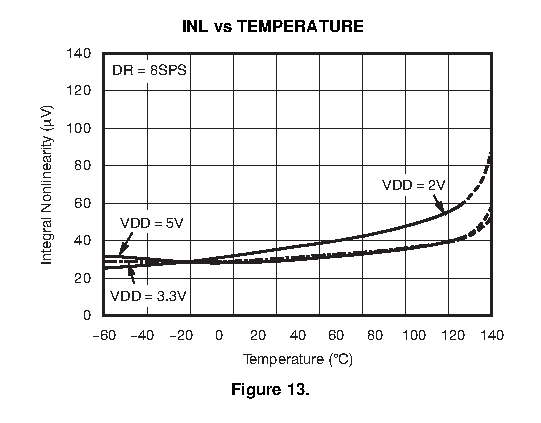
\includegraphics[width=\linewidth]{./my-chapters/my-images/ADC/datasheet_7.pdf}
	\end{minipage}
	\begin{minipage}{.5\linewidth}
		\begin{itemize}[label=+]
			\item Tại $T = 20^{o}C$: INL vs Temperature $= 22\,\mu\textsf{V}$
			\item Tại $T = 80^{o}C$: INL vs Temperature $= 38\,\mu\textsf{V}$
		\end{itemize}
	\end{minipage}
	
	\item Data Rate vs Temperature:
	
	\begin{minipage}{.5\linewidth}
		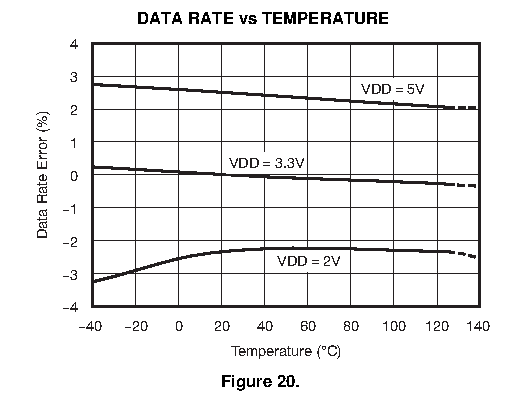
\includegraphics[width=\linewidth]{./my-chapters/my-images/ADC/datasheet_8.pdf}
	\end{minipage}
	\begin{minipage}{.5\linewidth}
		\begin{itemize}[label=+]
			\item Tại $T = 20^{o}C$: Data Rate Error $= 2.8\,\%$
			\item Tại $T = 80^{o}C$: Data Rate Error $= 1.2\,\%$
		\end{itemize}
	\end{minipage}
\end{itemize}

\subsection{Data Format}

Với ADS1115 là một ADC 16-bit với ngõ ra là một chuỗi bit có dấu theo giá trị như sau:

\begin{figure}[H]
	\centering
	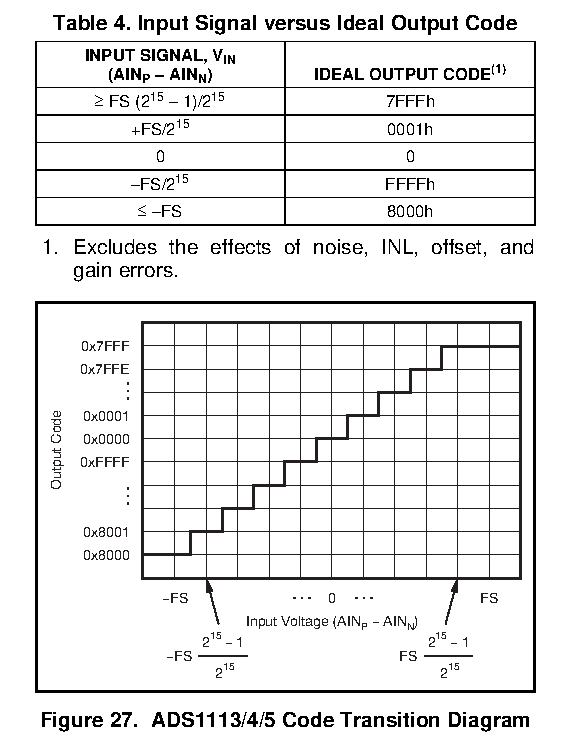
\includegraphics[width=.8\linewidth]{./my-chapters/my-images/ADC/datasheet_sampling.pdf}
	\caption{ADS1115 Code Transition Diagram.}
	\label{fig: CodeTransDiagram}
\end{figure}

Theo hình \ref{fig: CodeTransDiagram}, với $\textsf{FS} = 6.144$ như ở trên thì giá trị lớn nhất mà ADC có thể đọc được là $ V_{ref} \times \dfrac{2^{15} - 1}{2^{15}} \approx 6.1438\,\textsf{V}$ vẫn phù hợp với tầm đo là từ $0\rightarrow5 \,\textsf{V}$. Từ đó ta có công thức suy ngược từ $D_{out}$ nhận được từ ADC là:
\[ V_{out} = \dfrac{V_{ref}}{2^{15}} \times D_{out} = \dfrac{6.1438}{32768}\times D_{out} \]

\subsection{Kết quả của việc tính toán ADC}

Ta có bảng tính toán giá bên dưới, trong bảng giá trị có các giá trị như sau:

\begin{itemize}[label=-]
	\item \textbf{T\_s :} là giá trị nhiệt độ chuẩn cần đo.
	\item \textbf{V\_i :} là giá trị điện áp đo được từ sensor trong khoảng từ $0\rightarrow 5\,\textsf{V}$ với sai số là 5\%.
	\item \textbf{Offset\_Error :} là giá trị sai số của ADS1115 do nhiệt độ tạo nên.
	\item \textbf{Gain\_Error :} là giá trị của độ lợi của ADS1115 do nhiệt độ tạo nên.
	\item \textbf{V\_i\_ADC :} là giá trị mà ADC thực sự nhận tại chân \texttt{IN0}.
	\item \textbf{D\_out :} là giá trị tính toán từ giá trị điện đọc từ chân \texttt{IN0} với công thức là $\dfrac{V\_i\_ADC \times 2^{15}}{FS}$.
	\item \textbf{D\_cal\_Error :} là giá trị mà thực sự ADS1115 cho ra ở ngõ ra với các giá trị sai số cộng thêm do chính ADC và nhiệt độ.
	\item \textbf{Cal\_V :} là giá trị được tính trong MCU chuyển đổi từ giá trị Digital của ADS1115 gửi về cho MCU.
	\item \textbf{Cal\_Temp :} là giá trị chuyển đổi từ điện áp tính toán được \texttt{Cal\_V} về giá trị nhiệt độ theo công thức chuẩn là $T = \dfrac{V_{in} + \dfrac{5}{3}}{\dfrac{1}{2}}$.
\end{itemize}

\begin{landscape}
	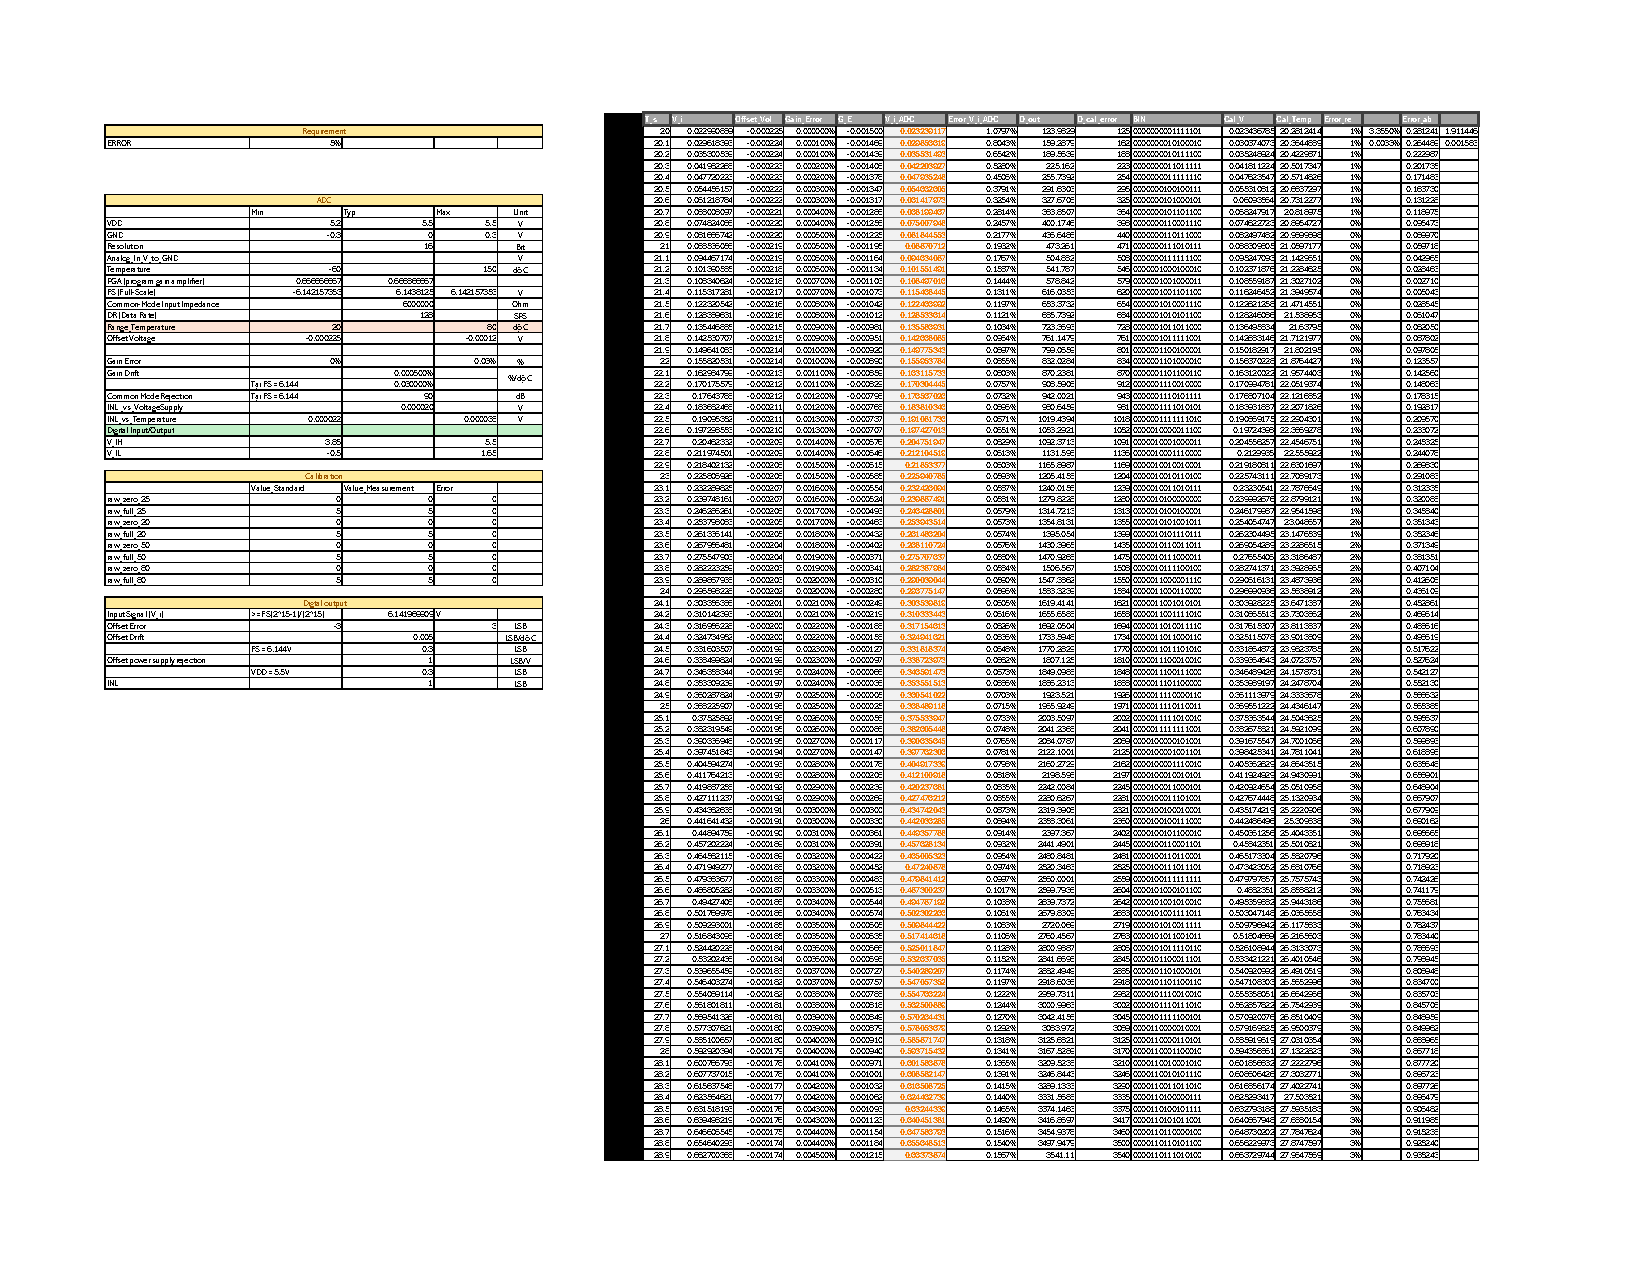
\includepdf[pages=-,angle=90,offset=0cm 0cm]{./my-chapters/my-images/ADC/Export_file_ADC.pdf}
\end{landscape}